\section{How the content is divided amongst the chapters}

Broadly, the thesis can be divided into three main parts: Introductions,  analytical results in relation to the Birth Death Catastrophe process,  and models of resulting from my curiosity.  Including this introduction and the conclusion,  these parts are divided amongst 8 chapters.  Below is a summary of the content and message of each.


\subsubsection{Chapter 2: Mathematical context}


Much of the work presented in this thesis surrounds topics of stochastic process theory,  and specifically branching processes.  Both continuous time and discrete time branching processes are examples of Markov chains exhibiting the Markov property: The probability of what happens next depends only on the current state of the system,   not on any past events;
\[
P(\xx_{t+1} = x_{t+1} \mid \xx_t = x_t, \xx_{t-1} = x_{t-1}, \ldots, \xx_0 = x_0) = P(\xx_{t+1} = x_{t+1} \mid \xx_t = x_t).
\] 
Continuous and discrete time Markov chains differ in their methods of analysis.  For example,  the fixation probabilities of discrete time processes can be understood using first step analysis which considers the single-step possible moves and their probabilities.  Continuous time chains on the other hand can be dealt with using the forward Kolmogorov Equation.  It is worth noting that continuous time chains can be "embedded" into discrete time versions by considering the probability distribution of \textit{next} events.  But when it comes to branching processes,  this fact shouldn't give the false impression that the two types of process are somehow identical in their dynamics,  just on modified time axes. Discrete time branching proceses differs fundamentally in that every individual either replicates or dies at once in each time step.  In the continuous time birth death process,  only single jumps up or down are possible at each move.  And this difference means there isn't a clear analyitical transformation between the two types of model.\par
It should be noted that we will only be dealing with discrete state space processes (jump chains).  Continuous state space models are also of interest, but the application to cellular replication nautrally lends itself to models with countable units. 
\vspace{10pt}

\noindent
One of the most important aspects of branching processes is their net replacement. This has slightly different interpretations in discrete and continuous time branching but esentially means the same thing.  It is the rate of change of the expected process count.  In discrete time: the expected number of offspring produced by a single individual in its lifetime.  
$$\mean{Z} = 2 p + 0(1-p) = 2p$$  
where p is the probability of an individual to replicate rather than die (wp $1-p$), and $Z$ is the number of offspring left by the one individual. \par 
In continuous time,  rate of population expansion,
$$\ddt{\mean{\xt}} = (\beta - \mu) \mean{\xt},$$
is quantified by $\beta - \mu$,  the net replication rate. 
In each case,  whether this number ($2p$ or $\beta - \mu$) is larger or less than 1 is of great signigicance. 


\begin{itemize}
\item When $2p$ or $\beta - \mu$ greater than 1,  the process is caled supercritical.  (see figure 1.2)
\begin{figure}[h!]
\centering
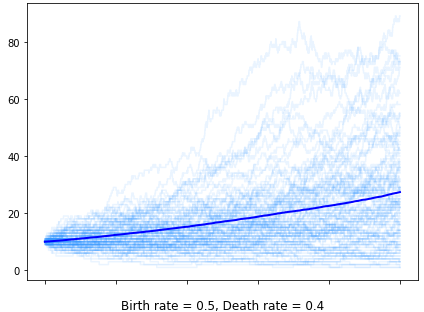
\includegraphics[width = 0.55\textwidth]{figures/fig_bd_regimes/BD54}
\caption{Supercritical birth death in continuous time.  In this and the following two figures, a large numer of individual realisations are shown in light blue, and their average is drawn in dark blue.  In each case, the sample mean shown forms a good approximation of the analytical mean.}
\label{im1}
\end{figure}
Some realisations die out, the rest continue rising towards infinity in an increasingly redictable exponential fashion. 
\end{itemize}


\begin{itemize}
\item When $2p$ or $\beta - \mu$ less than 1,  subcritical.  
\begin{figure}[h!]
\centering
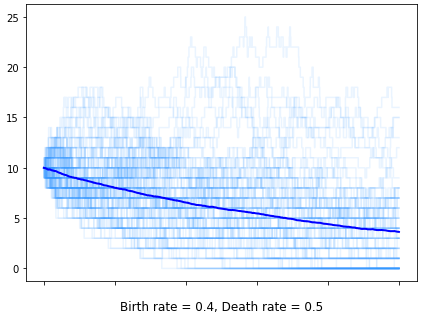
\includegraphics[width = 0.55\textwidth]{figures/fig_bd_regimes/BD45}
\caption*{Subcritical}
\end{figure}

All subcritical realisations are destined to die,  fixating at 0.


\end{itemize}


\begin{itemize}

\item And when $2p$ or $\beta - \mu$ is equal to 1,  the process is reffered to as critical.   

\begin{figure}[h!]
\centering
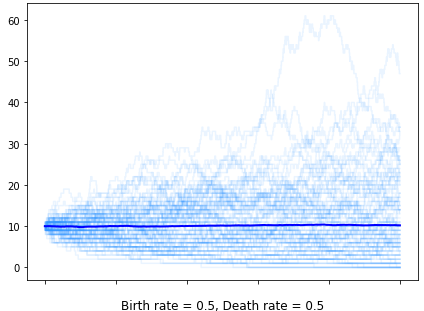
\includegraphics[width = 0.55\textwidth]{figures/fig_bd_regimes/BDpoint55}
\caption*{Critical}
\end{figure}

Line in the subcritical case, all critical realisations are destined to die out, but curiously, the expect time in which then do this is infinite.  A single process could possibly last for a very long time,  never fixating. 

\end{itemize}


\subsubsection{Chapter 3: Birth death catastrophe model -- main results}

This chapter introduces the Birth Death Catastrophe (BDC) process and outlines a series of results asociated with in. \par


\noindent
Around the 1980s, work was being done into growth models that incorporated stochastic declines (shocks). Out
of this came the the birth death catastrophe model as we know it \cite{cairns2004extinction}\cite{brockwell1985extinction} \cite{brockwell1982birth} \cite{dori2018family}.  An extension of the standard birth death
process, but where from every state apart from 0, a catastrophe event can take place, either causing a transition
to 0, or a special catastrophe state. Similar to birth and death events, this catastrophe state can be initiated by
any of the individual units, and so occurs with a rate proportional to the population size. We were interested
in this model for its potential application in modelling the development of an infection within cells that burst.
And more broadly, infections that spread amongst multiple cells.
Here the BDC model is defined and some key equations are introduced which describe the mean and variances
of the process. Some of the results have been found by others before, but we also have a few which extend beyond
the current literature. For example, we have a formula for the second moment of the process count in terms of the non-rupture probability. This, along with the process variance we found by solving a series of four ordinary differential equations.\par

Some attention is given to limiting conditional distributions. That is the behaviour of the process count assuming that by some late time fixation has not yet occurred.  We show that in some cases, quasi-stationarity is exhibited and we quantify the quasi-stationary mean as a function of rate parameters for replication and rupture.


\subsubsection{Chapter 4: Birth death catastrophe model -- additonal results}

This chapter extends the pervios one with more results,  especially those associated with state probabilities which are obtained from the forward Kolmogorov equation with the method of characteristics. 


\subsubsection{Chapter 5: Birth death catastrophe process -- modifications}

Here we explore the analytical possibilities of two modified BDC processes
\begin{itemize}
\item $\mathbf{N = 2}$ \textbf{sucessive imediate transfer}. We were generally interested in producing some kind of model which captured the dynamics of between-cell transfer and growth.  Moving in this direction,  we spent some time developing results in relation to the successive BDC process whereby a second process begins at the rupture of the first.  The anaysis didn't lead to exactly what we were looking for, but we found some distributions along the way,  and the work ultimately went on to lay the groundwork for the "fixed removal" model of chapter 6.   


\item \textbf{Two type}.  In 2011,  Antal and Krapivsky \cite{antal2011exact} published an exact solution to the two type continuouts time birth death process with one way mutation.  We were able to use their particular method, with some changes of variables,  to obtain the equivalent result for the two type BDC process.  This section simply outlines the process by which the result can be found. 


\end{itemize}


\subsubsection{Chapter 6: Bursting-budding comparrison}


Work has been done by others \cite{komarova2007viral} \cite{yuan2011stochastic} \cite{pearson2011stochastic} \cite{capistran2018extracellular} comparing the fundamental dynamical differences between budding and bursting style pathogenesis.  N. Komavora, for example proposed a potential advantage to busrting due to a flooding effect.  This chapter explores the significance of release counts when considering successive infiltration models.  That is, where pathogens go from one infected cell to another. \par
Each of the parts of this chapter consider he importance of locally depletable immune factors.  With only a finite supply of chalenges,  there is a sort of saftey in numbers effect.


\noindent
\textbf{Replicator suppressor}
This part considers the intracelllular environment in which there are toxin containing granules such as there are in macrophages and neutrophils.  Similar to a predetor pery model,  there are two individual types: replicators (pahogenic particles) and suppressors (granules).  It is clearly demonstratable that a larger incident population of replicators will have disproportonatly beter odds of survival and persistence in this case as more bacteria will be available to deplete the present immuno reserves. 


\noindent
\textbf{Fixed removal}
Moving from the intracellular to the extracellular environment. This part considers the question of how many released pathogenic particles manage to reach their next host.  In the extracellular medium between host cells there are a number of immune chalenges that the pathogens have to face. \par
For example,  complement proteins, which puncture bacterial cells deemed to be invaders,  and host bacteriophages which are viruses living in simbiosis with the organisms that may serve to kill forein agents. \par
The assumption is that these immune factors are locally depletable and that a larger group release of pathogens will somehow cause a flooding effect analogous to the one proposed by N. Komavora. 


\subsubsection{Chapter 7: Variability in evolution}
No topic has seduced and captivated my curiosity more than the question of what life is,  how it evolves,  and whether we can determine general underlying dynamics which uncover aspects fundamental to the reality of rise,  change,  and decay of living agencies. \par

Evolution into species, harbours a yet unsolved mystery to science.  We do know a lot.  For example,  vast efforts have been made in the last 5 decades into uncovering the microbiological mechanisms which underpin the replication and usage of DNA. \par


With regards to a big picture view,  progress is being made \cite{sharma2023assembly},  but we are yet to produce a widely taught and accepted description of what life is and how it changes which is consistent with concepts of neg-entropy production and thermodynamics more generally at the micro and macro scales. \par

But the hum and the buzz has been around for a while now,  and perhaps the writing is even on the wall as to how a water-tight conception might unfold.

Unfortunately,  this thesis does not have the answer.  Not only am I considerably under-qualified for the task,  but this project was supposed to be about Yersinia Pestis,  and it largely is.  Of course,  Y.  pestis bacteria is one of the most acute examples of a living dissipative structure.  \par

\vspace{10pt} 


\noindent
 Mostly before the PhD and in the first year,  I read a few books which went on to change the way I thought about science,  philosophy,  and particularly the topic of evolution.  Most significantly: 


\begin{itemize}
\item \textbf{Order out of chaos,  Mans new dialogue with nature --  Ilya Prigogine and Isabelle Stengers,  1984}
Outlines the theory of dissipative structures -- chaotic order formations which take place as local reductions in entropy in the as a means of dissipation in the context of a wider increase in entropy consistent with the second law \cite{prigogine2018order}.

\item \textbf{What is life -- Erwin Schrödinger, 1944}
Frames the problem of understanding what life is in the context of energy gradients,  neg-entropy and the laws of thermodynamics \cite{schrodinger1946life}.   

\item \textbf{Chance and necessity -- Jacques Monod, 1970}
Overviews the (at the time) new understanding of DNA molecular biology and mechanisms of replication and transcription \cite{monod1974chance}.  Then explores the concept of teleology and what it means for living objects, made of mere chemistry, to have volition. \par 
Outlines animism and vitalistic schools of thought and belief.

\item \textbf{The genetical theory of natural selection -- Ronald Fisher, 1930}
Covers the topic of evolution broardly from a mathematical perspective. Then goes on to discuss the implications of birth rates being different among sectors of society.  Also the rise and fall of civilisations. \cite{fisher1929genetical}. 

\item \textbf{Wonderful life -- Stephen J Gould, 1990}
All about the Cambrian explosion,  a geologically instantaneous period of a few million years in which great diversification of species took place.  Contrasting the previous Ediaceran fauna of docile wandering discs of the sea floor, all of a suden, there were a vast array of segmented athropodic forms.  Displaying arms, legs, eyes, mouths and claws;  eating one another and josstling for survival in what must have been a tropical tempo of savage egoisms \cite{gould1989wonderful}. 

\item \textbf{Beyond good and evil -- Friedrich Nietzsche}
Covers a wide range of topics surrounding, from the historical development of moralities to the emergence of species in relation to environmental conditions and suspended potential within a population.  \cite{nietzsche2013beyond}

\item \textbf{(Some of) On the origin of species -- Charled Darwin, 1859}
Needs no introduction.  Hard to read though with the old timey langauge style! Mostly interested in what he said of rate of variation in cases of domesticated animals.  \cite{darwin1859origin} 
\end{itemize}


They drew my attention to fact that the rate of evolution and divergence into species,  among other things,  is driven by a combination of selective pressures and energy availability.  For example,  the presence of competing species and how much food is readily available for a given population in its ecosystem.  It seems that these two factors make up a kind of push-pull tension,  simultaneously holding a group together with the necessity to conform so as to be strong in the face of competition for survival; whilst constantly pulling it apart with the ravenous impulse of variation which is a natural component of living matter as consistent with the second law of entropy increase. \par

Nietzsche writes about this sort of dynamic in ``Beyond good and evil" section 262:

\begin{quotation}
\noindent
"A species arises, a type becomes fixed and strong through protracted struggle against essentially constant unfavourable conditions. Conversely, one knows from the experience of breeders that species which receive plentiful nourishment and an excess of care and protection soon tend very strongly produce variation of their type and are rich in marvels and monstrosities"
\end{quotation}

\noindent
Sexual selection also offers a mystery in this space.  It seems to both macroscopically bring a population together through mixing of traits whilst also (microscopically) introducing disorder into genomes crossed over.  I won't attempt to make heads or tails of this apparently confusing juxtaposition.  Maybe someone else has and perhaps it isn't as confusing as it may appear. \par 

\vspace{10pt}

\noindent
 
\noindent
But my suspicion is that there is a underlying dynamic to articulate.  That there is a building of tension,  and release at the advent of more favourable circumstances.  And that this takes place in a cyclic fashion across multiple domains. \par

That this release is as it were more dissipative,  and during it,  when there is a greater fanning out of forms,  that this is an example of a dissipative structure which produces a chaotic formation of complex order in the form of bifurcating species and forms.  Sort of as in fluid turbulence bifurcating fluid trajectories create a chaotic dissipation of heat through friction.  The analogy is albeit more artistic than scientific,  but fun to think about! \par
If we consider the example of planar flow around a circle,  there is here this property of a cyclic to and fro -- flow speeding up followed by turbulence shedding,  low pressure and repetition. 

\vspace{8pt}
\hrule 
\vspace{8pt}
\noindent
\textbf{Bit of an aside:} I can't help but be interested in the possibility that this sort of speculated dynamic could be used to apocryphally explain cultural trends in societies.  One potential example is the apparent trend for strict conservative values to become prevalent after a period of substantial economic and cultural dynamism which ultimately brought about liberal tolerance.\par

It could be hypothesised that this has happened at least twice before in history: In Iraq and the middle east more broadly after its golden age of expansion in the first few centuries of the second millennium, and also in Sumatra and Java of Indonesia in the 16th century after the eventual decline of the Hindu kingdoms.  (The Hindu court culture was all pushed to Bali where it survived -- see David Attenborough's 1969 documentary "The miracle of Bali",  It's not particularly relevant to the point,  but definitely worth a watch anyway).  Note: I only discovered the theorey of anacyclosis \cite{podes1991polybius} after writing this, but there appears to be some similarity. 

\begin{figure}[h!]
\centering
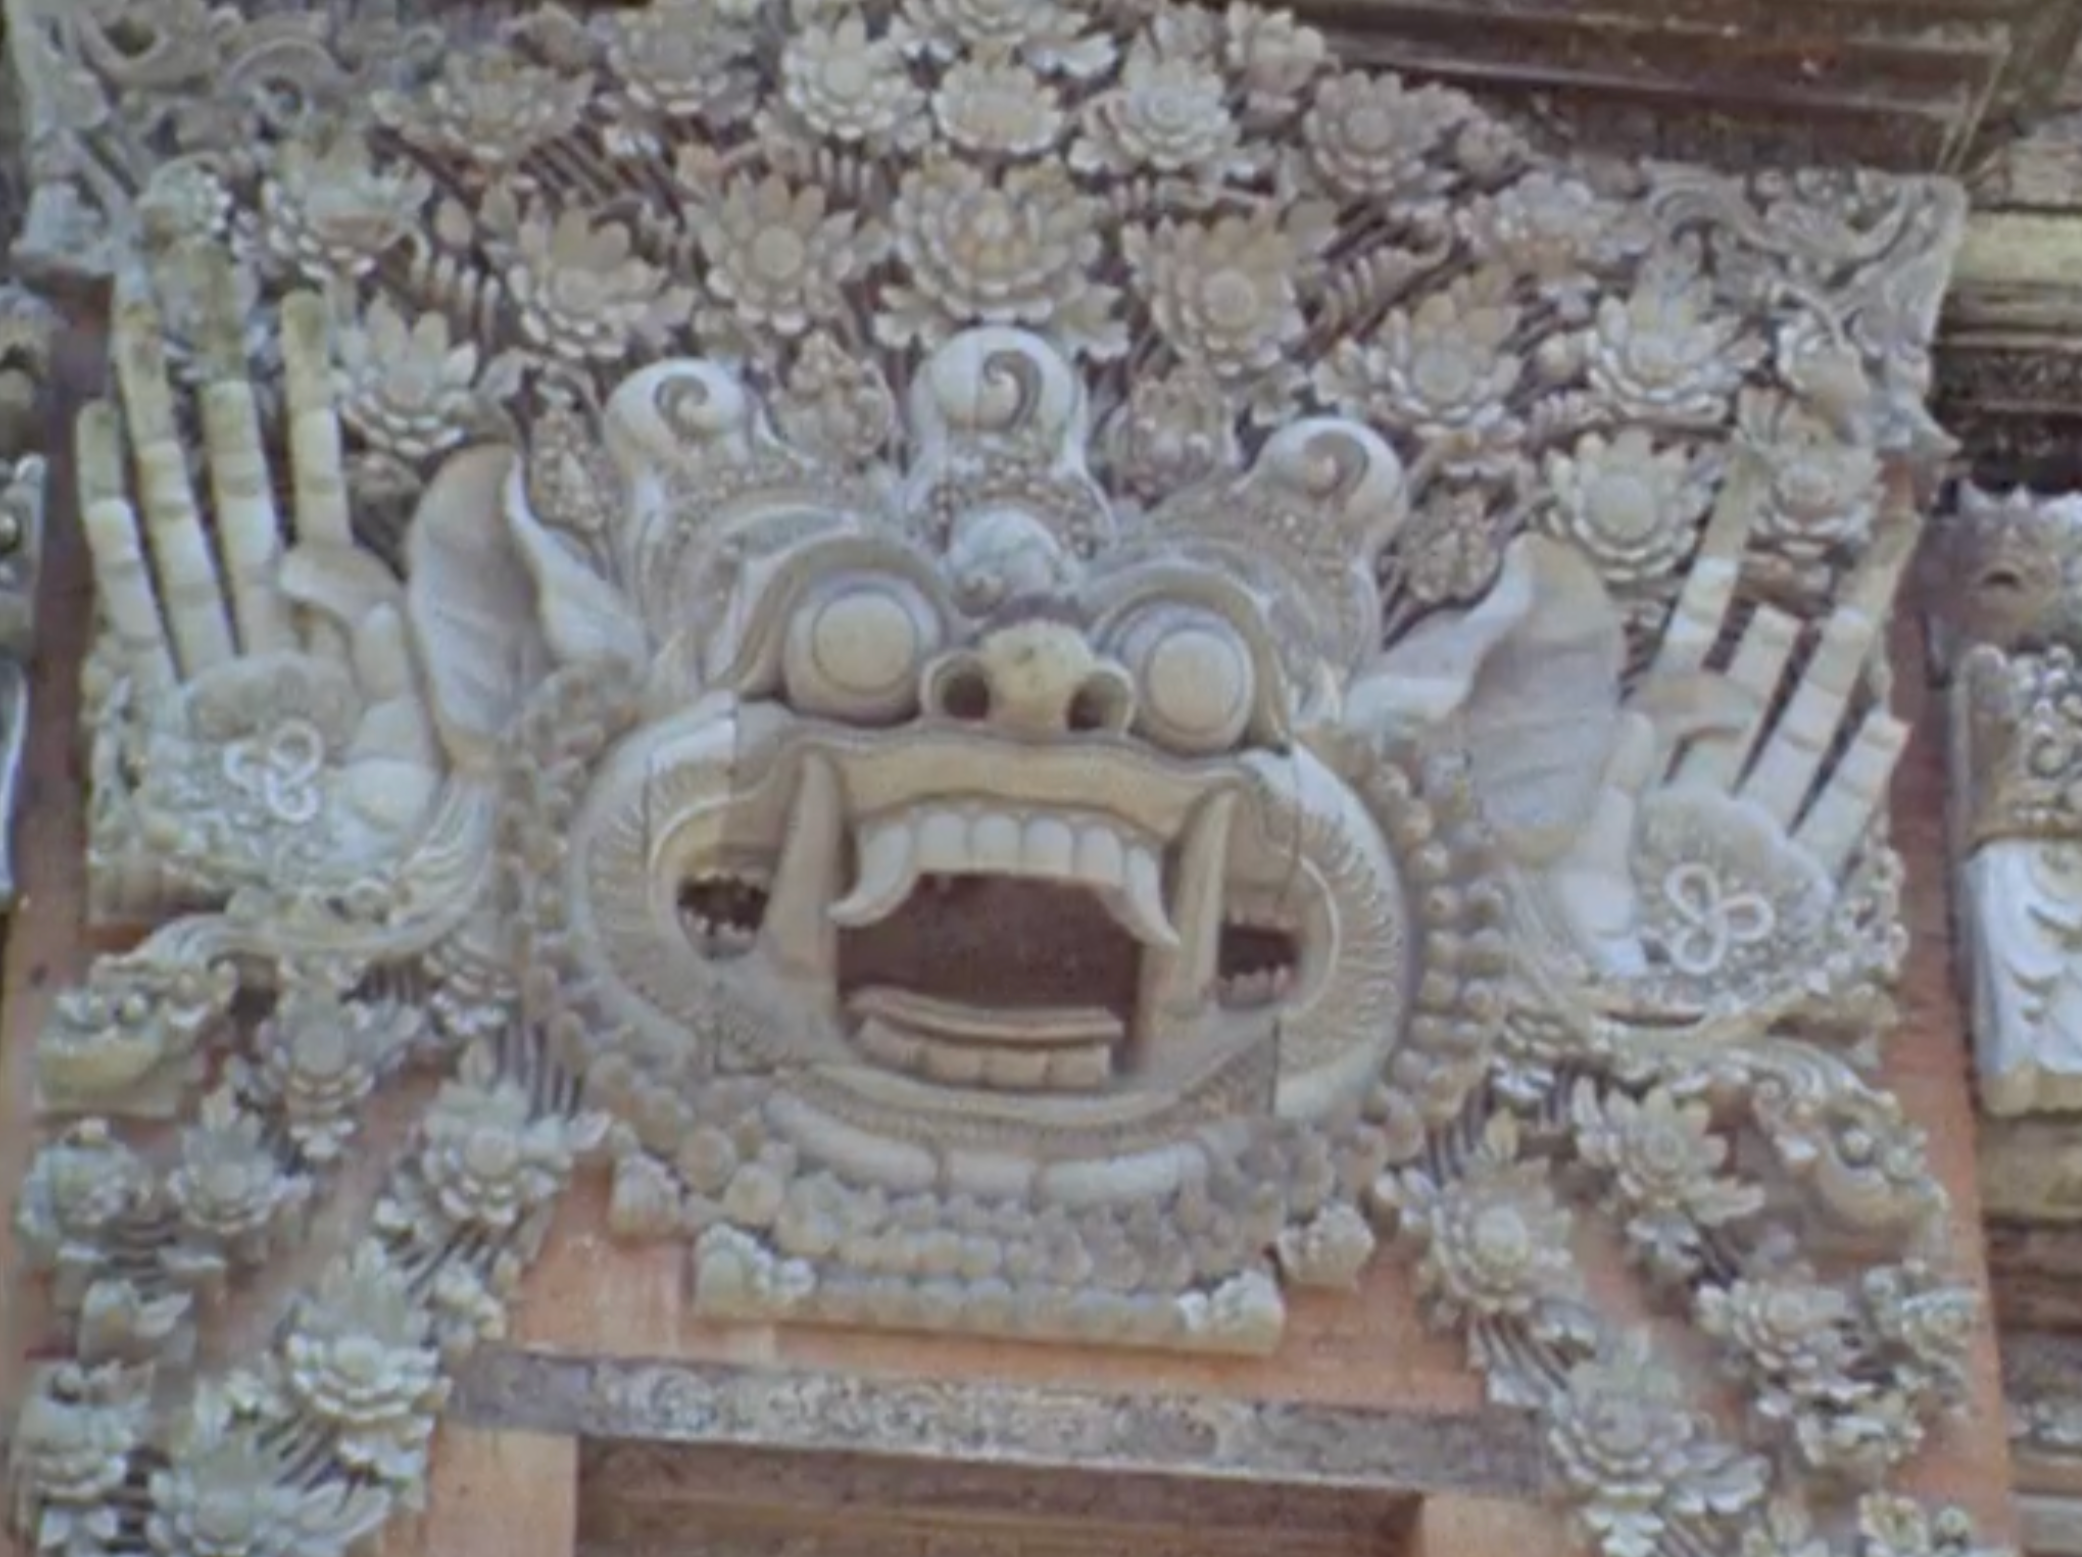
\includegraphics[width = 0.8\textwidth]{figures/fig_bali/bali}
\caption*{A carved image on the wall of a Balinese temple. Interesting how the face appears threatening, whilst also being surrounded by an emination of flowers. }
\end{figure}

\vspace{8pt}
\hrule
\vspace{8pt}

The content of this chapter is divided into two key sections accompanied by some more vapid topics of a more divergent nature.  Here is outlined the two key parts: 

\begin{itemize}
\item  \textbf{ Logistic speciation} In the spirit of Yule's 1924 paper and other more recent work with birth death processes, \cite{nee1994extinction} a continuous time Markov chain is formulated to model the production of species within a genus.  This model differs from the standard birth death process by having an inhomogeneous origination rate.  That is, the rate at which new species emerge is a function of time 
$$\beta(N(t)) $$
which is based on the relative availability of resources for a genus population which is expanding into a domain. The logistic model is used to describe the size of the population $N(t)$ in relation to its carrying capacity,  $K$  and this relative difference is taken to form the basis of the origination rate $\beta$. 


\item \textbf{ Pimentel fly model (cyclic competitive exclusion)}
"The ecological theatre and the evolutionary play" (G.  E.  Hutchinson) contains a summary of an experiment done by someone called Pimentel in the 50s.  It's purpose was to challenge the theory of competitive exclusion which states that two species can not simultaneously occupy the same niche.  It showed that an oscillation can arise when two species of fly occupy the same space provided that travel through the space is slowed by a series of compartments within the container.  This being because when one species gets pushed to near extinction,  it evolves more in response to infraspecific competitive interactions than those interspecific interactions with members of its group. \par 
This part of the chapter is about a model of these observed dynamics.\par
I also propose an addition to this model which aims to mirror the dynamic talked about in the Nietzsche quote (speciation being more prevalent when the species is the dominant of the two). 


\item \textbf{Allegorical model of rise run ruin and rejuvenation}
This is a model of one of the more vapid areas of this chapter.  The concept includes a quantity aiming to quantify potential (or vitality) in the system. This quantity,  $N(t)$ being high drives the emergence of species $\xt$.  But then, high $\xt$ count has the effect of reducing the potential.  Eventually as the quantity of allowance of "potential" per species $N/\xt$ becomes particularly low (its inverse being high), the rate of catastrophe increases to the point of certain collapse,  whereby $\xt$ declines suddenly to 0.  Subject then only to Poisson revival.  \par 

This is set up with the aim of representing something like the cyclic dissipative pattern of bifurcations seen in the example of stokes flow around a circle (oscillating turbulence shedding), and might also be seen in the rise and (sometimes sudden) fall of structures such as civilisations (speaking with reckless apocryphal speculation).  

\end{itemize}


\begin{figure}[h!]
\centering
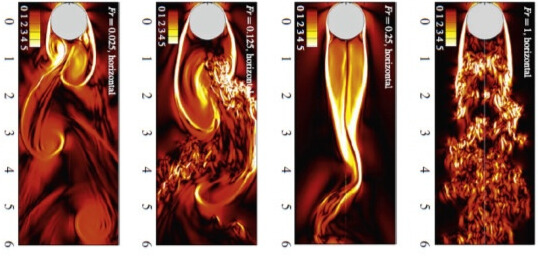
\includegraphics[width = 0.8\textwidth]{figures/fig_stokes/Stokes}
\caption*{Stokes flow around a circle with cyclic turbulence shedding.}
\end{figure}


\subsubsection{Chapter 8: Conclusion}


This chapter begins with the pursuit of a curiosity.  The question of whether a replication rate advantage, weighted towards the beginning of a branching process will lead it to generally outperform another process without the front weighting.  I should specify that a condition is imposed whereby the two compared models have overall the same "replicative potential".  In the case of discrete time branching, this condition manifests in the sum of the dividing probabilities being the same over a defined number of generations. \par 

\vspace{10pt}
\noindent
The reason for this curiosity was to determine whether there is some fundamental advantage to replication being weighted towards the outset.  It turns out not to be the case; there is no advantage (in the expected value at least), provided the condition. \par 

In the case of Y. pestis seeking a replicative advantage in host macrophages,  the condition of equivalent overall replicative potential of course doesn't hold.  Because taking the higher rate at the outset doesn't diminish the rate of extracellular replication. \par 
The next part of this chapters explores stochastic birth death style models which encorporate two phases.


\vspace{15pt}
\noindent
\textbf{Two phase models}
The first phase in each of the following models represents the pro-phagocytosis phase of Y. pestis pathogenesis.  The second phase represents extracellular growth. \par

A few versions are explored: 

\begin{itemize}
\item \textbf{Birth-death to birth-death}
With two successive birth death processes, the duration of the first can be controlled directly as a parameter.  And this indirectly controlls the initial count in the second phase.


\item \textbf{Birth-death-catastrophe to birth-death-catastrophe}
In the case of an initial BDC process followed by birth death, the duration of the first phase is determined indirectly by the bursting rate. 

\item \textbf{Constant to birth-death}
Here,  the initial count of the second phase is controlled directly. This is the same as what was described in part of the the Mathematical bacground section (demonstrating the importance of initial counts in slightly supercrictical birth death processes).  The closer to criticallity (from above) the process, the more significant the effect.  And it seems straightforward to argue (which I hope to do elsewhere) that most biological replication processes,  if they are supercritical at all, opperate close to the critical threshold. (This is of course excepting cases where the early stages of a logistic groth phase are still causing more substantially exponential growth). 


\item \textbf{Constatnt to birth-subdusive-death}  A subducive death rate simply means a death rate which declines as a function of time.  This assumption follows loosly from a theory that over time, Y. pestis will after progresing through more and more generation cycles, begin to adapt to the particular environment of that host.  The presence of host-symbiotic immuno bacteriophages could form the basis of an example in which this dynamic applies.  In other words, the first Y. pestis may not be able to subvert the attacks of certain present bacteriophages, but maybe its great grandaughter can.  \par 
If a dynamic like this were present, it could have the effect of causing the extracellular net-replication rate to begin sub-critical, and tend into supercriticallity over time. In this case, a larger initial cohort would be of vital importance,  this possibly being provided by the within macrophage phase. 
\end{itemize}


\noindent
\textbf{Quadrant argument}
There is a simple argument for why Y.  pestis would favour phagocytosis to begin with and an anti-phagocytosis strategy  when neutrophil recruitment takes place: That neutrophils are more effective killers,  and so Y. pestis would want to avoid them.  But why not resist phgocytosis to begin with? Likely because the macrophage intracellular environment permits some replicative advantage. This section mathematizes this straightforwad argument using the simple birth death process.
